\documentclass{article}
\usepackage[T1]{fontenc}
\usepackage{lmodern}
\usepackage{graphicx}
\usepackage{amsmath,amssymb}
\usepackage[a4paper,margin=2cm]{geometry}
\usepackage[absolute,overlay]{textpos}
\setlength{\TPHorizModule}{1mm}
\setlength{\TPVertModule}{1mm}
\usepackage[indonesian]{babel}
\usepackage{hyperref}
\setlength{\emergencystretch}{2em}
% unit: Halaman 28

\begin{document}

% === Halaman 28 (llm) ===

\begin{center}
\Large Mode CBC
\end{center}

\vspace{60mm}

\begin{tabular}{|c|c|c|}
\hline
CBC & $\begin{aligned} C_1 &= E(K, [P_1 \oplus IV]) \\ C_j &= E(K, [P_j \oplus C_{j-1}]) \ j = 2, \dots, N \end{aligned}$ & $\begin{aligned} P_1 &= D(K, C_1) \oplus IV \\ P_j &= D(K, C_j) \oplus C_{j-1} \ j = 2, \dots, N \end{aligned}$ \\
\hline
\end{tabular}

% deskripsi: Diagram proses enkripsi dan dekripsi menggunakan mode Cipher Block Chaining (CBC). Bagian (a) menunjukkan proses enkripsi di mana plaintext di-XOR dengan IV atau ciphertext sebelumnya sebelum dienkripsi. Bagian (b) menunjukkan proses dekripsi di mana ciphertext didekripsi terlebih dahulu lalu di-XOR dengan IV atau ciphertext sebelumnya untuk mendapatkan plaintext.
% bbox normalisasi: [0.0180, 0.2800, 0.9820, 0.6300]
\begin{textblock*}{202.44mm}(3.78mm,83.16mm)
\noindent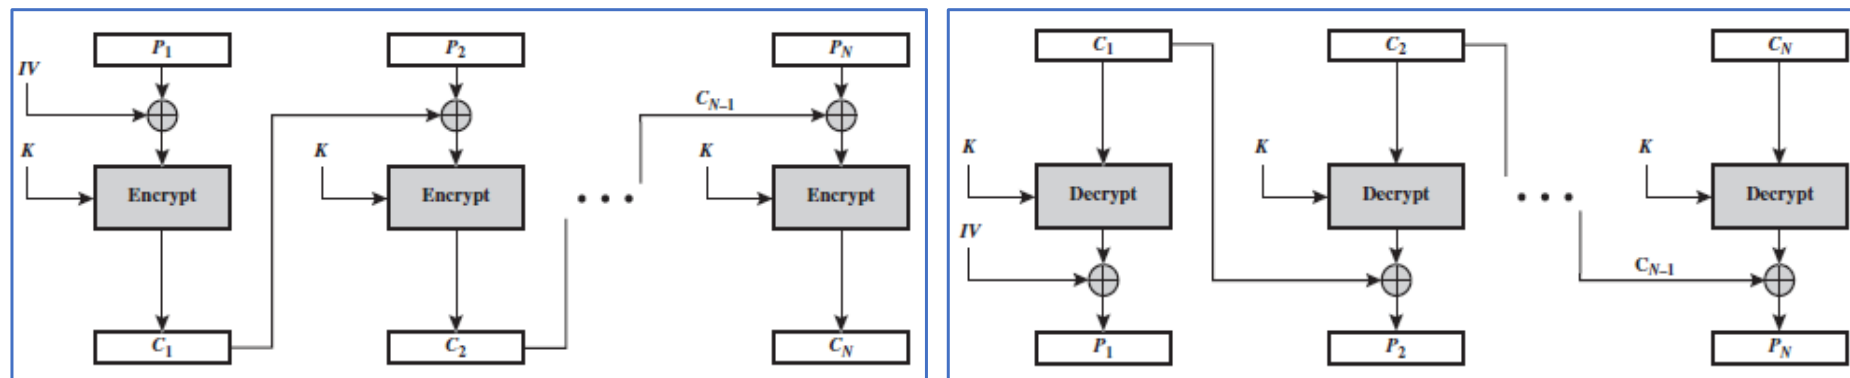
\includegraphics[width=202.44mm,height=103.95mm]{../../images/llm/page_028_img_01.png}%
\end{textblock*}

\end{document}
